\documentclass[conference]{IEEEtran}

\usepackage{cite}
\usepackage{amsmath,amssymb,amsfonts}
\usepackage{algorithmic}
\usepackage{graphicx}
\usepackage{textcomp}
\usepackage{xcolor}
\def\BibTeX{{\rm B\kern-.05em{\sc i\kern-.025em b}\kern-.08em
    T\kern-.1667em\lower.7ex\hbox{E}\kern-.125emX}}
    
\usepackage{lipsum}

\usepackage{listings}
\lstset{
    basicstyle=\scriptsize \ttfamily ,
	escapeinside=``,
	linewidth=\textwidth,
	numbers=left,
	numberstyle=\footnotesize  \ttfamily \color{blue},
	%frame=trbl,
	breaklines=true,
	aboveskip=1em,
	framextopmargin=2pt,framexbottommargin=2pt,abovecaptionskip=-3pt,belowcaptionskip=3pt,
} %Required for inserting code

\def\figurewidth{0.45\textwidth}
\graphicspath{{figure/}}
\usepackage[hidelinks]{hyperref}

\usepackage{caption}
\usepackage{subcaption}


\begin{document}

\title{Report: Experiment on Cloud Computing \thanks{This experiment was funded by the course of Cloud Computing and Huawei's Collegiate Education Program "Zhineng Jizuo".}}

\author{\IEEEauthorblockN{Victrid}
\IEEEauthorblockA{\textit{dept. of Computer Science and Engineering} \\
\textit{Shanghai Jiao Tong University}\\
Shanghai, China \\
\href{https://github.com/Victrid}{github.com/Victrid}}
}

\maketitle

\section{Introduction}
As computer technology continues to cross into various fields, the resulting huge amount of data makes it challenging to analyze and process the data. Traditional single computer programs have difficulty processing these data, while mainframe clusters are expensive and require complex operations and controls, making them limited to large analytics companies.

Today, cloud computing technology is reaching into every corner of the world. As the superiority of controlled cost, elastic management, and rapid migration is gradually being demonstrated, even ordinary people are able to access these resources and take advantage of them. The development of distributed technology has also made it possible to process huge amounts of data on inexpensive computer arrays. Today's cloud computing centers have become an important part of the Internet's infrastructure and will occupy an even more important position in the future.

This report on Cloud Computing Experiment contains these parts:

\begin{itemize}
    \item Create VM cluster and configure Hadoop and Spark framework on Huawei Cloud.
    \item Run The Examples from Hadoop and Spark.
    \item Solve actual problems with GraphX API with Spark.
\end{itemize}

\section{Configuration of Virtual Machine Cluster}

\subsection{Mirror Configuration}

Fast provisioning and delivery, automation, and ease of scaling are key to today's elastic computing. However, setting up instances one by one, configuring their cumbersome dependencies and environment variables, and installing them by downloading source code and binary packages from the web and configuring them by copy and paste is typical of UNIX mainframe administrators in the 1980s.

Compared to the handbook \cite{li-chao} suggests that using an Ubuntu image and configure them manually, we've built a custom mirror, which already has Hadoop, Spark, and SBT packed up and modified. We referenced the image creation tool provided by Arch Linux on \cite{Arch-box} with the Cloud-init tool and rewrote the compiling script of the Hadoop package on \cite{hadoop-package} to match the \texttt{JAVA\_HOME} lookup process. A system installation script was written to suit the needs of this experiment. This series of configuration files are placed in the submitted files' \texttt{image-buildscript} folder.

Many cloud providers has provided custom image service, so do Huawei Cloud. By utilizing its IMS services \cite{IMS} as figure \ref{fig:ims}, we can now create virtual machines with our pre-built images.

\begin{figure}[ht]
    \centering
    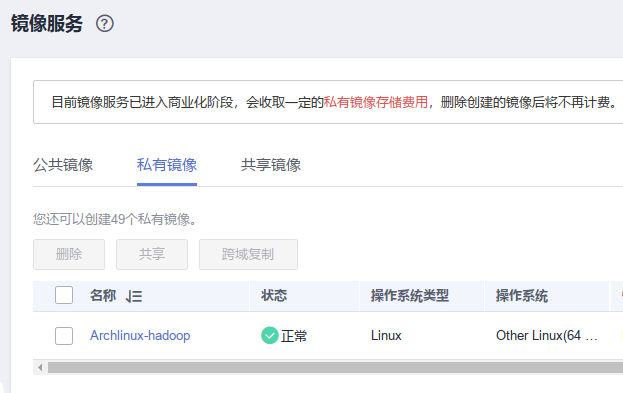
\includegraphics[width=\figurewidth]{figure/hadoop-image.png}
    \caption{Huawei Cloud IMS}
    \label{fig:ims}
\end{figure}

\subsection{Virtual Machine Configuration}

To perform VM configuration as designed in our mirror, adjusting roles while the VM is created, we use Huawei Cloud SDK and its OpenAPI to perform creation. The core part is to utilize OpenStack \texttt{user\_data}. When the \texttt{user\_data} is provided as bash scripts, it will be run at VM creation by cloud-init. The script we created performs Hadoop configuration according to Hadoop Documentation \cite{Hadoop-setup}, worker appointment, and SSH key configuration. This series of configuration scripts and API call Python scripts are placed in the submitted files' \texttt{HuaweiCloud-openAPI} folder.

\subsection{Hadoop Initiation}

By running the commands below: (Our Hadoop instance is installed under \texttt{/usr/lib})

\begin{verbatim}
cd /usr/lib/hadoop
bin/hdfs namenode -format
sbin/start-all.sh   
\end{verbatim}

The Hadoop instance will be set up, and can be viewed via \texttt{http://master:9870} as in figure \ref{fig:DN-info}.

\begin{figure}[ht]
    \centering
    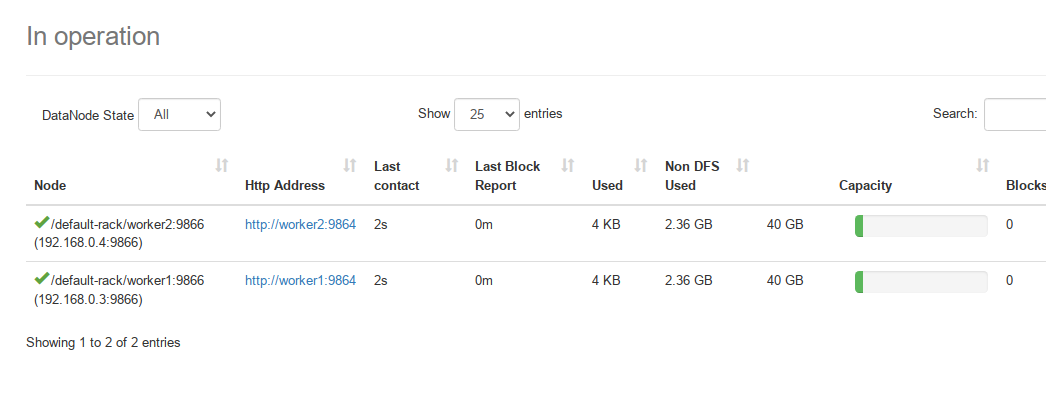
\includegraphics[width=\figurewidth]{figure/configured-hadoop.png}
    \caption{DataNode Information on NameNode}
    \label{fig:DN-info}
\end{figure}

\section{Hadoop Example: wordcount}

We've prepared a dummy text file, containing \emph{lorem ipsum}, an industry standard dummy text in the printing and typesetting since 1500s. The text file contains 150 paragraphs, 13547 words, and is used to test.

The text file is transmitted to the master node via \texttt{scp} at \texttt{/root/lorem.txt}.

by running the commands below (at \texttt{/root} folder):

\begin{verbatim}
hadoop fs -mkdir /input
hadoop fs -put lorem.txt /input
hadoop jar /usr/lib/hadoop/share/hadoop/\
mapreduce/\
hadoop-mapreduce-examples-3.3.1.jar \
wordcount /input /output
hadoop fs -cat /output/part-r-00000
\end{verbatim}

The running results are shown in figure \ref{fig:word-count}. Both input file and results are put in the \texttt{WordCount} folder.

\begin{figure}[ht]
    \centering
    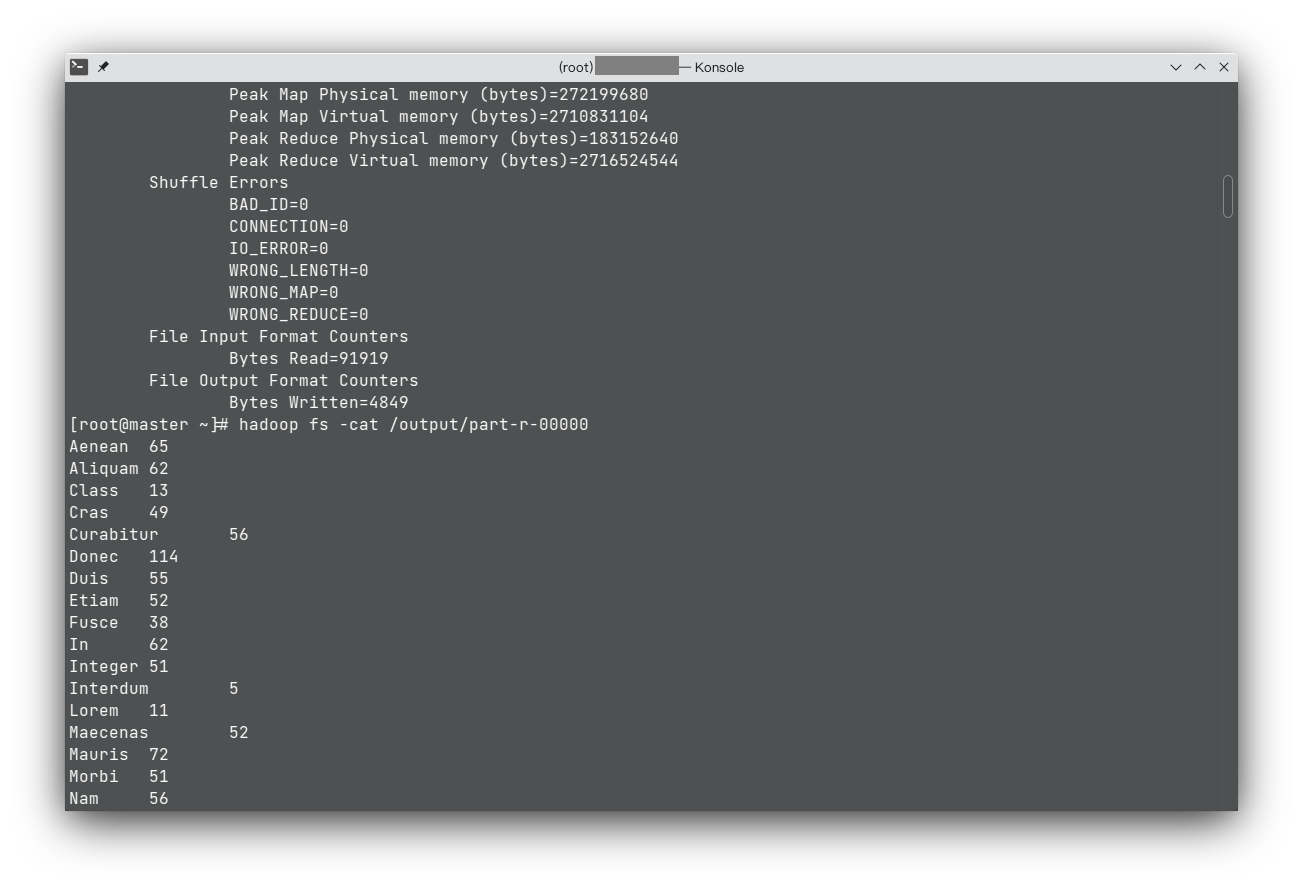
\includegraphics[width=\figurewidth]{figure/word-count.png}
    
    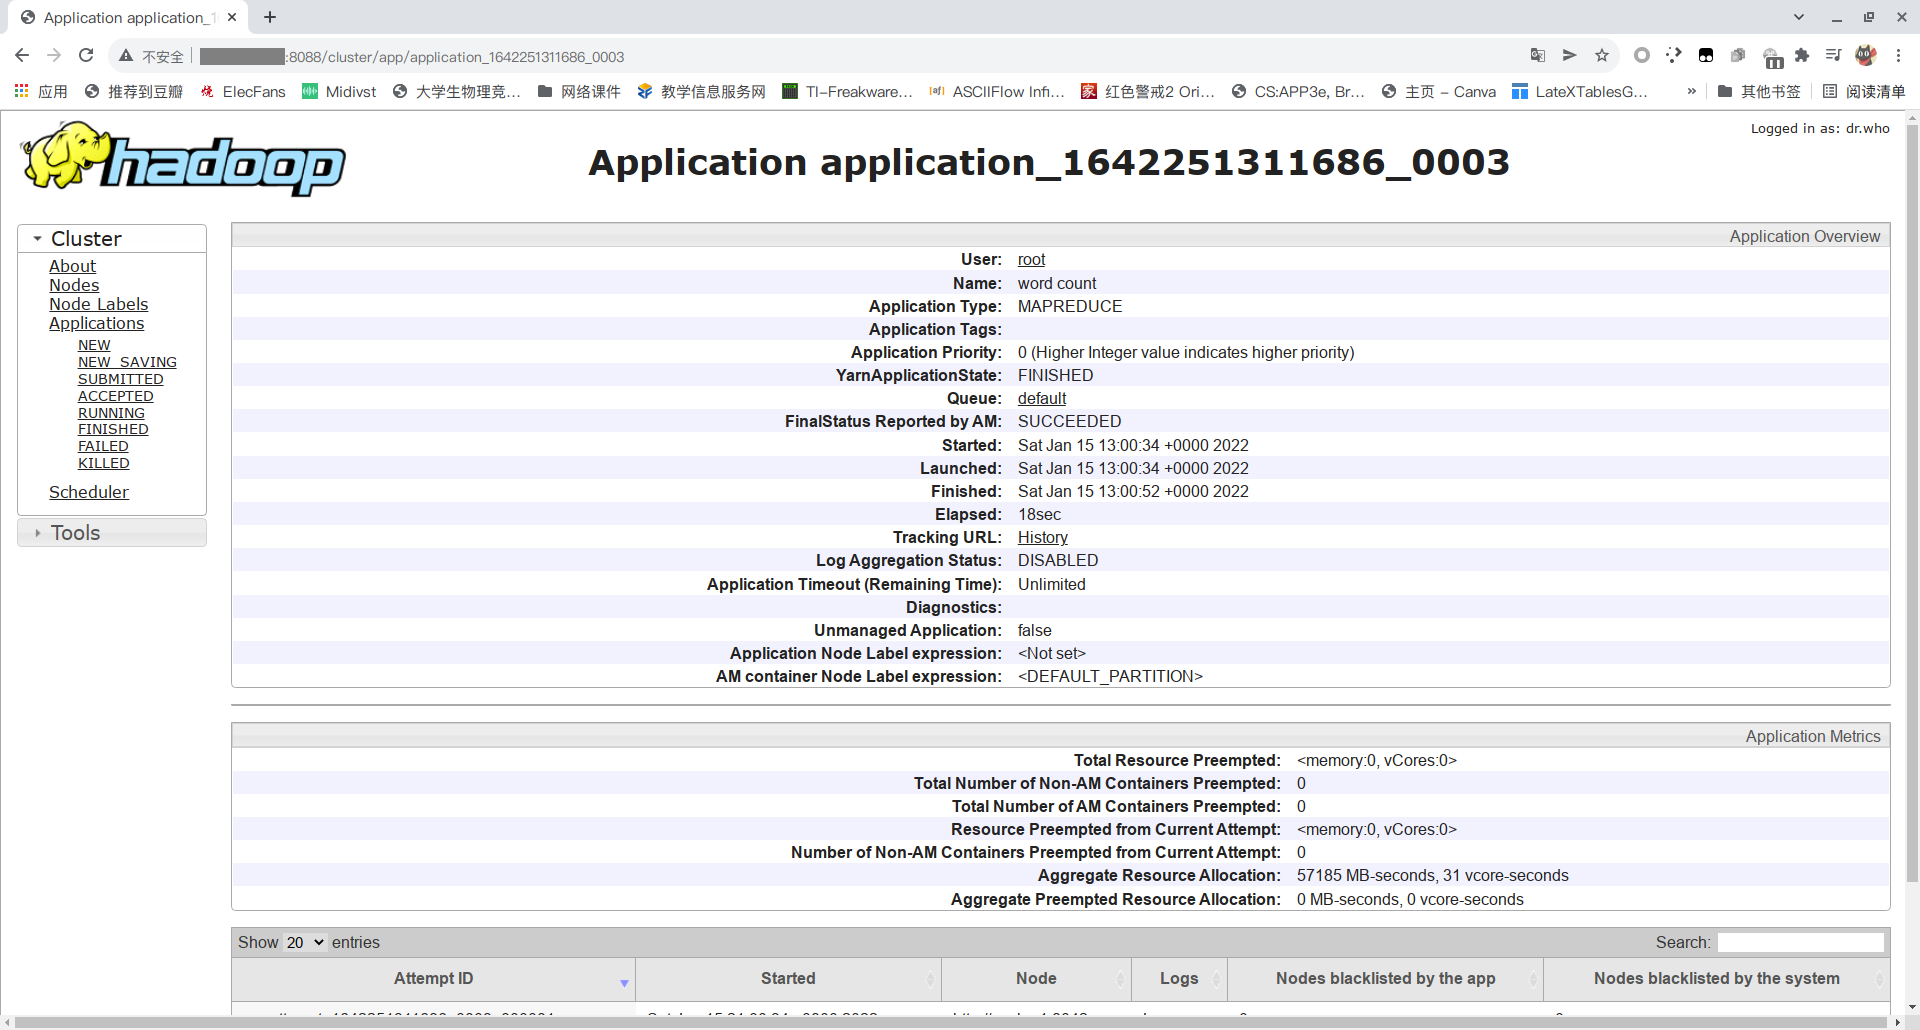
\includegraphics[width=\figurewidth]{figure/mapreduce.png}
    \caption{Word Count Results}
    \label{fig:word-count}
\end{figure}

By running the commands below, we can clear the input files and results. This will be helpful for further experiments.

\begin{verbatim}
hadoop fs -rm -f -r /output
hadoop fs -rm -f -r /input
\end{verbatim}

\section{GraphicX Example: Connected Component}

We've copied the needed file and organized as \cite{xmu-spark}. The package needs more dependencies than WordCount program, and the scala used by Spark 3.2.0 should be 2.12.15. We modified the simple build tools script as below:

\begin{verbatim}
#    [Trailed for PDF typesetting]
scalaVersion := "2.12.15"

libraryDependencies+="org.apache.spark" \
    %% "spark-core" % "3.2.0"
libraryDependencies+="org.apache.spark" \
    %% "spark-sql" % "3.2.0"
libraryDependencies+="org.apache.spark" \ 
    %% "spark-graphx" % "3.2.0"
\end{verbatim}

After compiling as in figure \ref{fig:compile}, we upload these 2 graph txt files to data/graphx folder on HDFS, and call the class by \texttt{org.\allowbreak{}apache.\allowbreak{}spark.\allowbreak{}examples.\allowbreak{}graphx.\allowbreak{}ConnectedComponentsExample} as in figure \ref{fig:spark-submit} and received the result as in figure \ref{fig:spark-result}:

\begin{verbatim}
(justinbieber,1)
(matei_zaharia,3)
(ladygaga,1)
(BarackObama,1)
(jeresig,3)
(odersky,3)
\end{verbatim}

The necessary files and source code are put in the \texttt{GraphX} folder.

\section{PageRank Algorithm}

Here we use the Wikipedia Vote Network dataset \cite{wikipedia} as our processing source. The requested PageRank algorithm is similar to the \emph{Connected Component} one, and after checking the spark source code, we're sure that the \texttt{GraphLoader} can also be used to process the wiki votes.

PageRank algorithm is named after both the term "web page" and Google co-founder Larry Page. The key to the ranking is a probabilistic balance between nodes. At the beginning of the computational process the pagerank for each node is randomized, and for each iteration, the rank is computed as:

\begin{equation}
PR(p_i) =\frac{1-d}{N} + d\sum_{p_j\in M(p_i)}\frac{PR(p_j)}{L(p_j)}
\end{equation}

An approximation of real page rank value can be calculated with several iterations.

After researching on GraphX Programming Guide \cite{pagerank}, the graph build with GraphLoader has implemented PageRank algorithm. In our implementation, it is called by

\begin{verbatim}
val ranksGraph = graph.pageRank(0.0001)
\end{verbatim}

The original source file does not contain name information, but we want to form a more intuitive result as \emph{Connected Component}, which adds an additional user--node linkage. We used \texttt{sed} scripts to pre-process the original vote data from \cite{wiki-elec}, and generate the user--node list as in \texttt{users.txt}.

{\small
\begin{verbatim}
sed '/^[\s]*#/d; 
/^\s*$/d;
/^[ET].*/d; 
/^N\t-1\tUNKNOWN.*/d;
s/^[UN]\t\(.*\)\t\(.*\)$/\1,\2/g;
s/^V\t.*\t\(.*\)\t.*\t\(.*\)$/\1,\2/g' \
original.txt | sort -g | uniq > users.txt
\end{verbatim}
}

The user--node list generated would be like:

{\small
\begin{verbatim}
3,ludraman
4,gzornenplatz
5,orthogonal
6,andrevan
7,texture
8,lst27
9,mirv
...
\end{verbatim}
}

After compiling and submitting like we've done in the \emph{Connected Component} part, the results are shown below and as figure \ref{fig:PR-result}:

{\small
\begin{verbatim}
PR: 32.78, ID:4037, Name:elonka
PR: 26.18, ID:  15, Name:danny
PR: 25.52, ID:6634, Name:tenpoundhammer
PR: 23.36, ID:2625, Name:_clown_will_eat_me
PR: 18.56, ID:2398, Name:werdna
PR: 17.96, ID:2470, Name:alex_bakharev
PR: 17.76, ID:2237, Name:khoikhoi
PR: 16.14, ID:4191, Name:ryulong
PR: 15.44, ID:7553, Name:dihydrogen_monoxide
PR: 15.30, ID:5254, Name:gracenotes
PR: 14.51, ID:2328, Name:phaedriel
PR: 14.48, ID:1186, Name:william_m._connolley
PR: 13.84, ID:1297, Name:robchurch
PR: 13.78, ID:4335, Name:mer-c
PR: 13.75, ID:7620, Name:cobi
PR: 13.65, ID:5412, Name:protectionbot
PR: 13.57, ID:7632, Name:redirectcleanupbot
PR: 13.33, ID:4875, Name:earle_martin
PR: 12.87, ID:6946, Name:useight
PR: 12.69, ID:3352, Name:crzrussian
\end{verbatim}
}

Although we do not know how Wikipedia administrators are selected, after checking their usernames, those we checked were all engaged in Wikipedia administration during 2008. This shows that distributed computing is not just an airy idea in papers or academics, but can also work well in solving practical problems.

All necessary files and source code are put in the \texttt{PageRank} folder.

\newpage
\section{Conclusion}
\emph{Omitted}.

\vfill
\bibliographystyle{IEEEtran}
\bibliography{reference}

\clearpage
\onecolumn
\section*{Supplementary}
\begin{figure}[ht]
     \centering
     
     \begin{subfigure}[b]{0.48\textwidth}
         \centering
        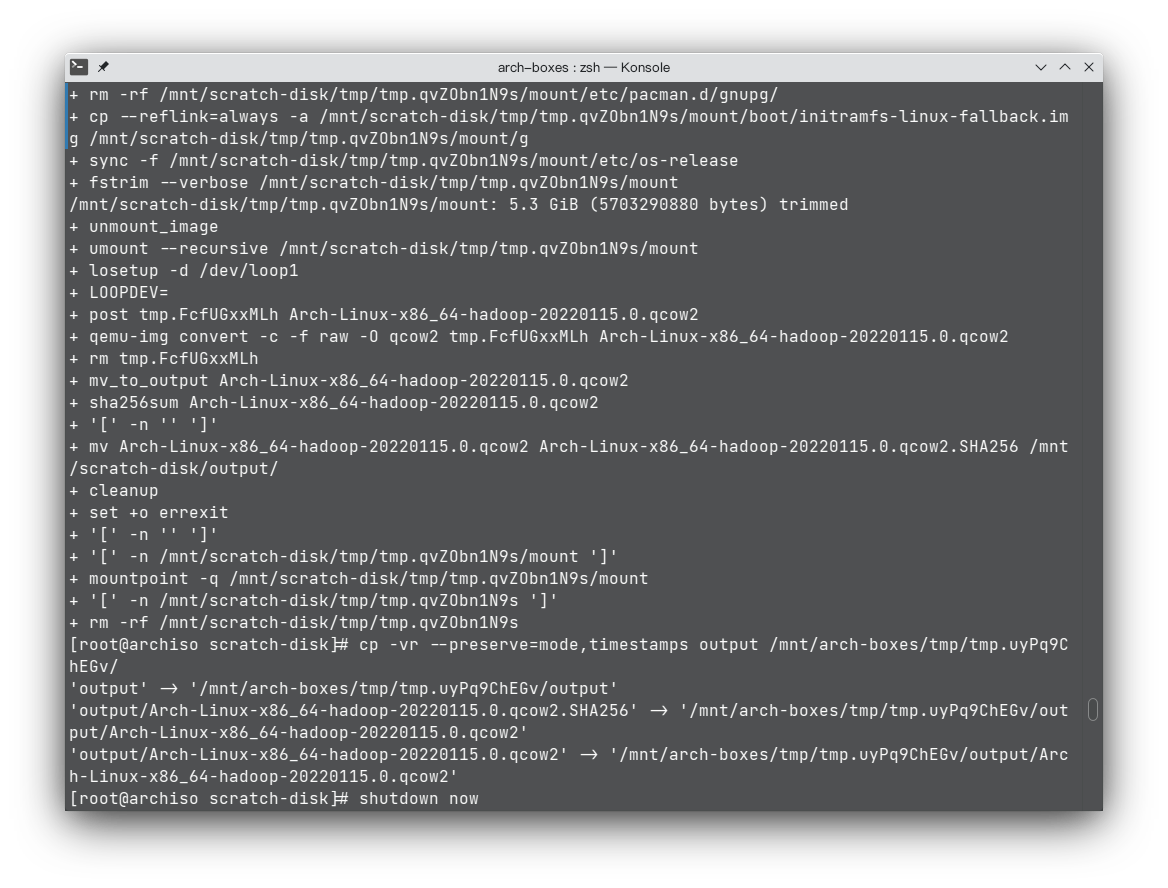
\includegraphics[width=\textwidth]{figure/build-images.png}
        \caption{Building Images}
        \label{fig:build-img}
     \end{subfigure}
     \begin{subfigure}[b]{0.48\textwidth}
         \centering
    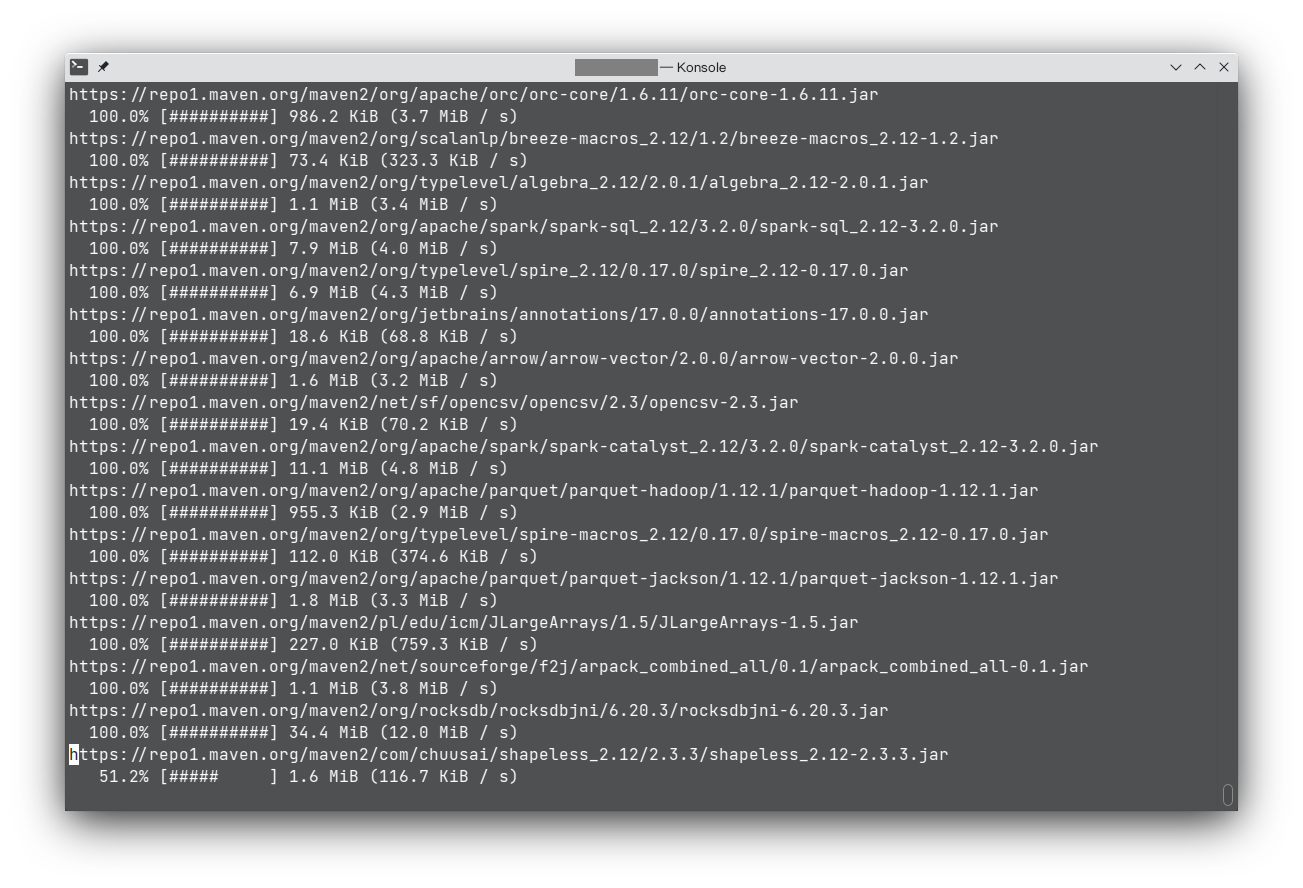
\includegraphics[width=\textwidth]{figure/compiling.png}
    \caption{SBT compilation}
    \label{fig:compile}
     \end{subfigure}
     
     \begin{subfigure}[b]{0.48\textwidth}
         \centering
    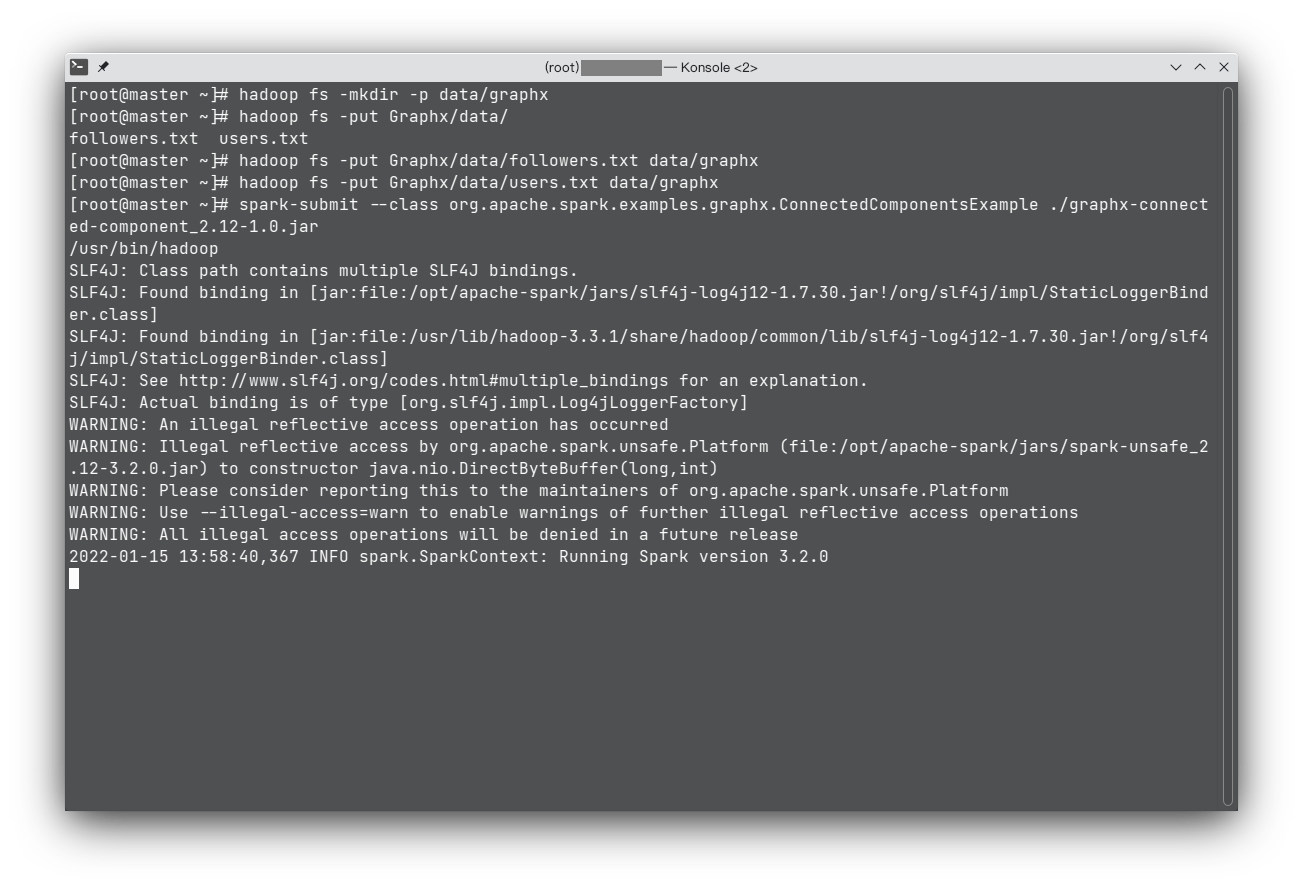
\includegraphics[width=\textwidth]{figure/spark-submit.png}
    \caption{Spark Submission}
    \label{fig:spark-submit}
     \end{subfigure}
     \begin{subfigure}[b]{0.48\textwidth}
         \centering
    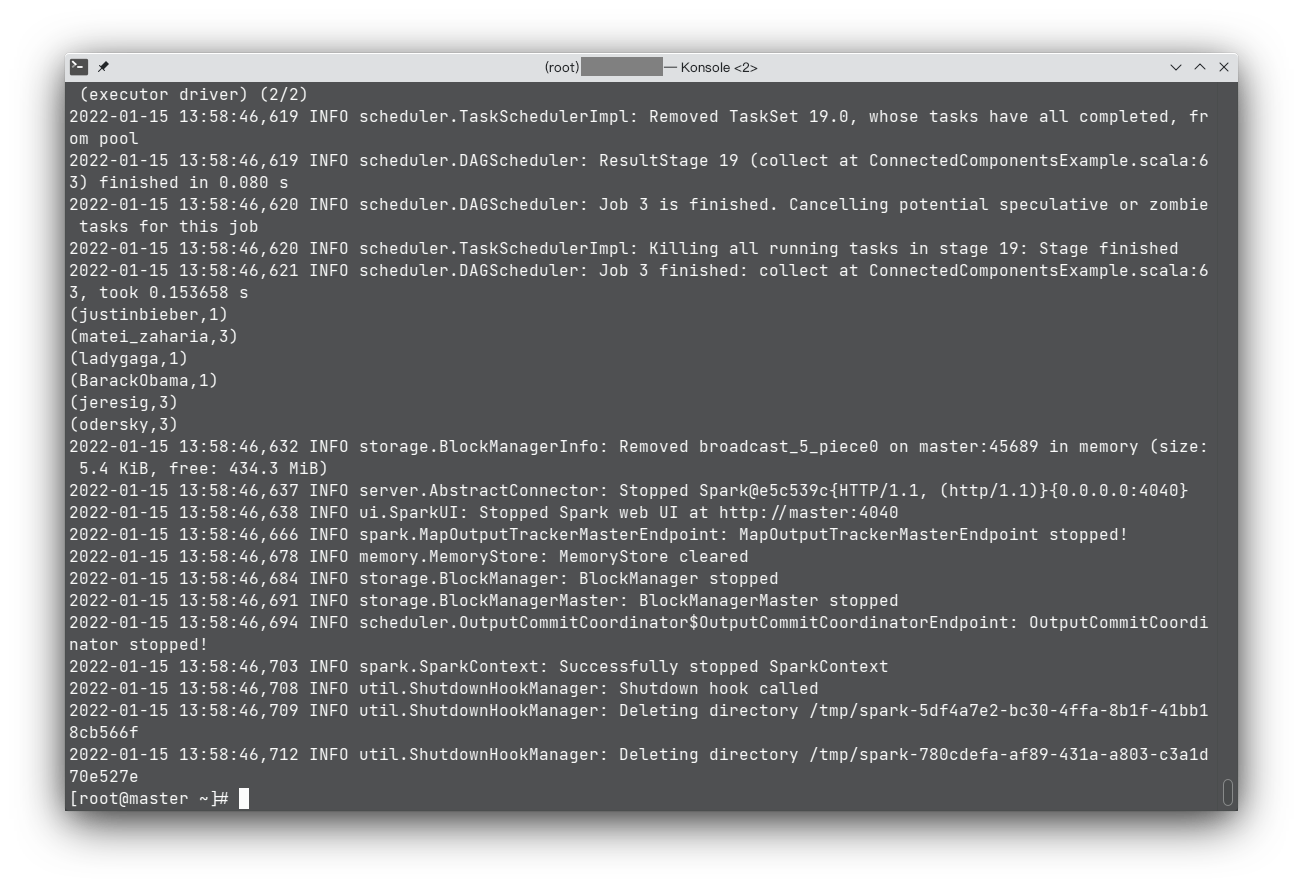
\includegraphics[width=\textwidth]{figure/spark-result.png}
    \caption{Spark GraphX results}
    \label{fig:spark-result}
     \end{subfigure}
     
     \begin{subfigure}[b]{0.48\textwidth}
         \centering
    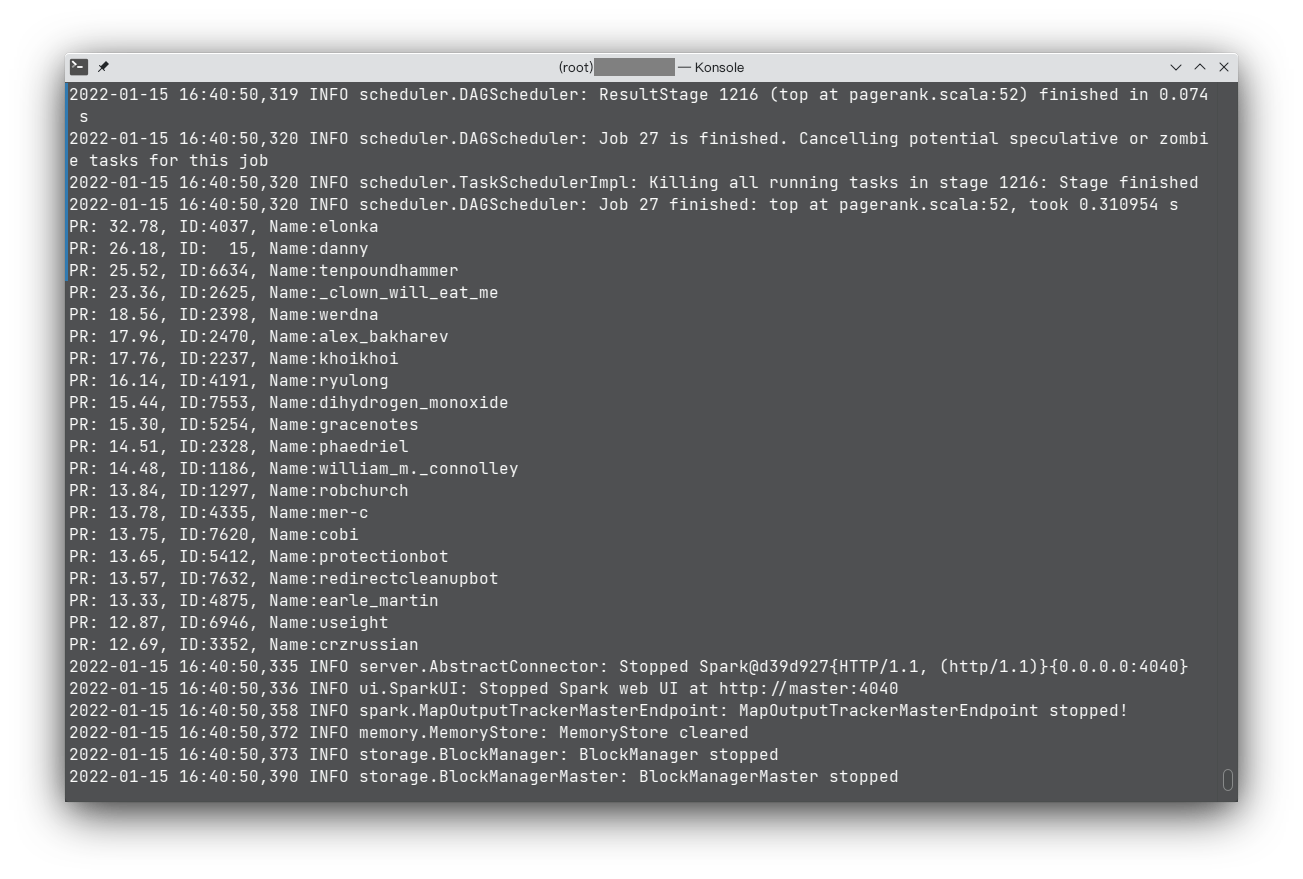
\includegraphics[width=\textwidth]{figure/PR-result.png}
    \caption{Page Rank results}
    \label{fig:PR-result}
     \end{subfigure}
     
        \caption{Supplementary Figures}
        \label{fig:supp}
\end{figure}


\end{document}
